\newpage
\chapter{Ensayo de impulso (1,2/50 \textmu s)}
\vspace{3\baselineskip}

El presente capítulo establece el marco normativo del ensayo de impulso de alta tensión, estableciendo conceptos básicos, y los parámetros característicos de la onda de impulso atmosférico tipo rayo \qty[parse-numbers=false]{1,2/50}{\micro\second}. 

\section{Definiciones normativas}
\label{sec:definiciones_normativas}

Los siguientes términos son un extracto en la norma IEC 60060-1 \cite{iec60060_1}:

\textbf{Tensión de impulso:} Es una tensión transitoria aperiódica aplicada intencionalmente, que usualmente se eleva rápidamente a un valor de cresta y luego cae más lentamente a cero.

\textbf{Tensión de impulso tipo rayo:} Es una tensión de impulso con un tiempo de frente inferior a 20 µs.

\textbf{Tensión de impulso tipo rayo completa:} Es una tensión de impulso tipo rayo, que no es interrumpida por una descarga disruptiva.
\begin{figure}[H]
    \centering
    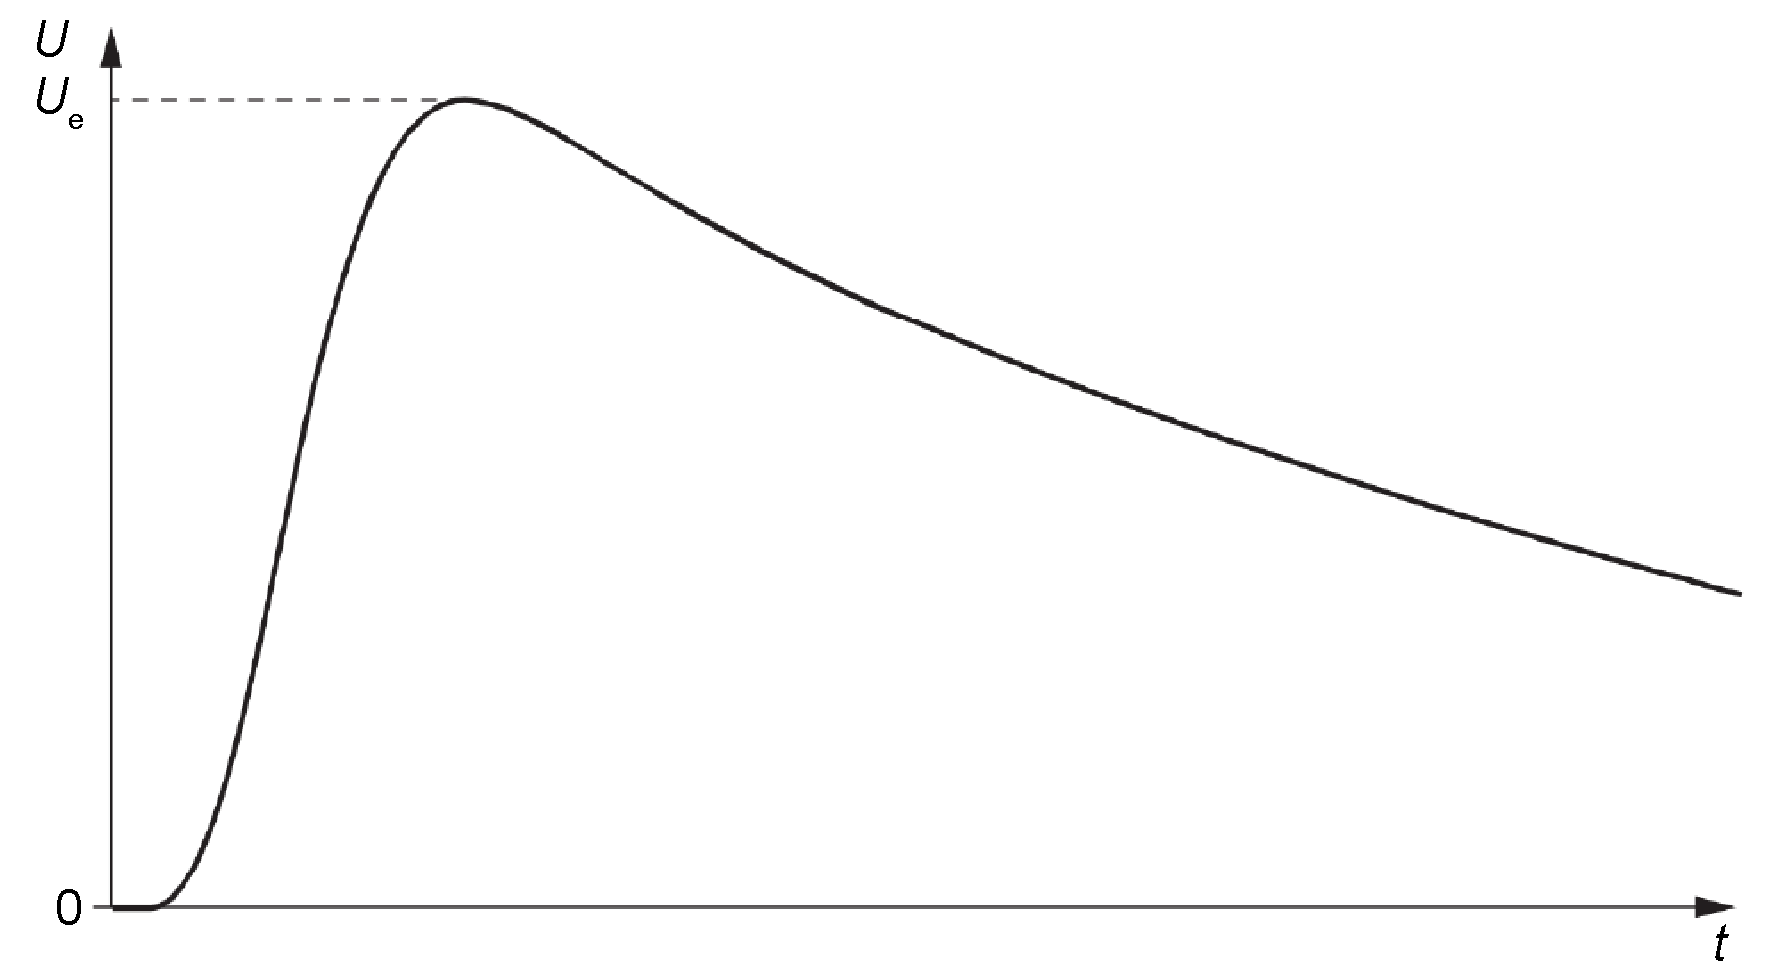
\includegraphics[width=1\textwidth]{img/iec_60060_1_impulso_tension_pleno.png}
    \caption{Impulso de tensión tipo rayo pleno.}
    \label{fig:impulso_tension_pleno}
\end{figure}

\textbf{Sobreelevación / oscilación (overshoot):} Es un incremento de la amplitud de una tensión de impulso debido a una oscilación amortiguada en la cresta, causada por el circuito.

\textbf{Curva registrada:} Es una representación gráfica o digital de los datos de ensayo de una tensión de impulso.
\begin{figure}[H]
    \centering
    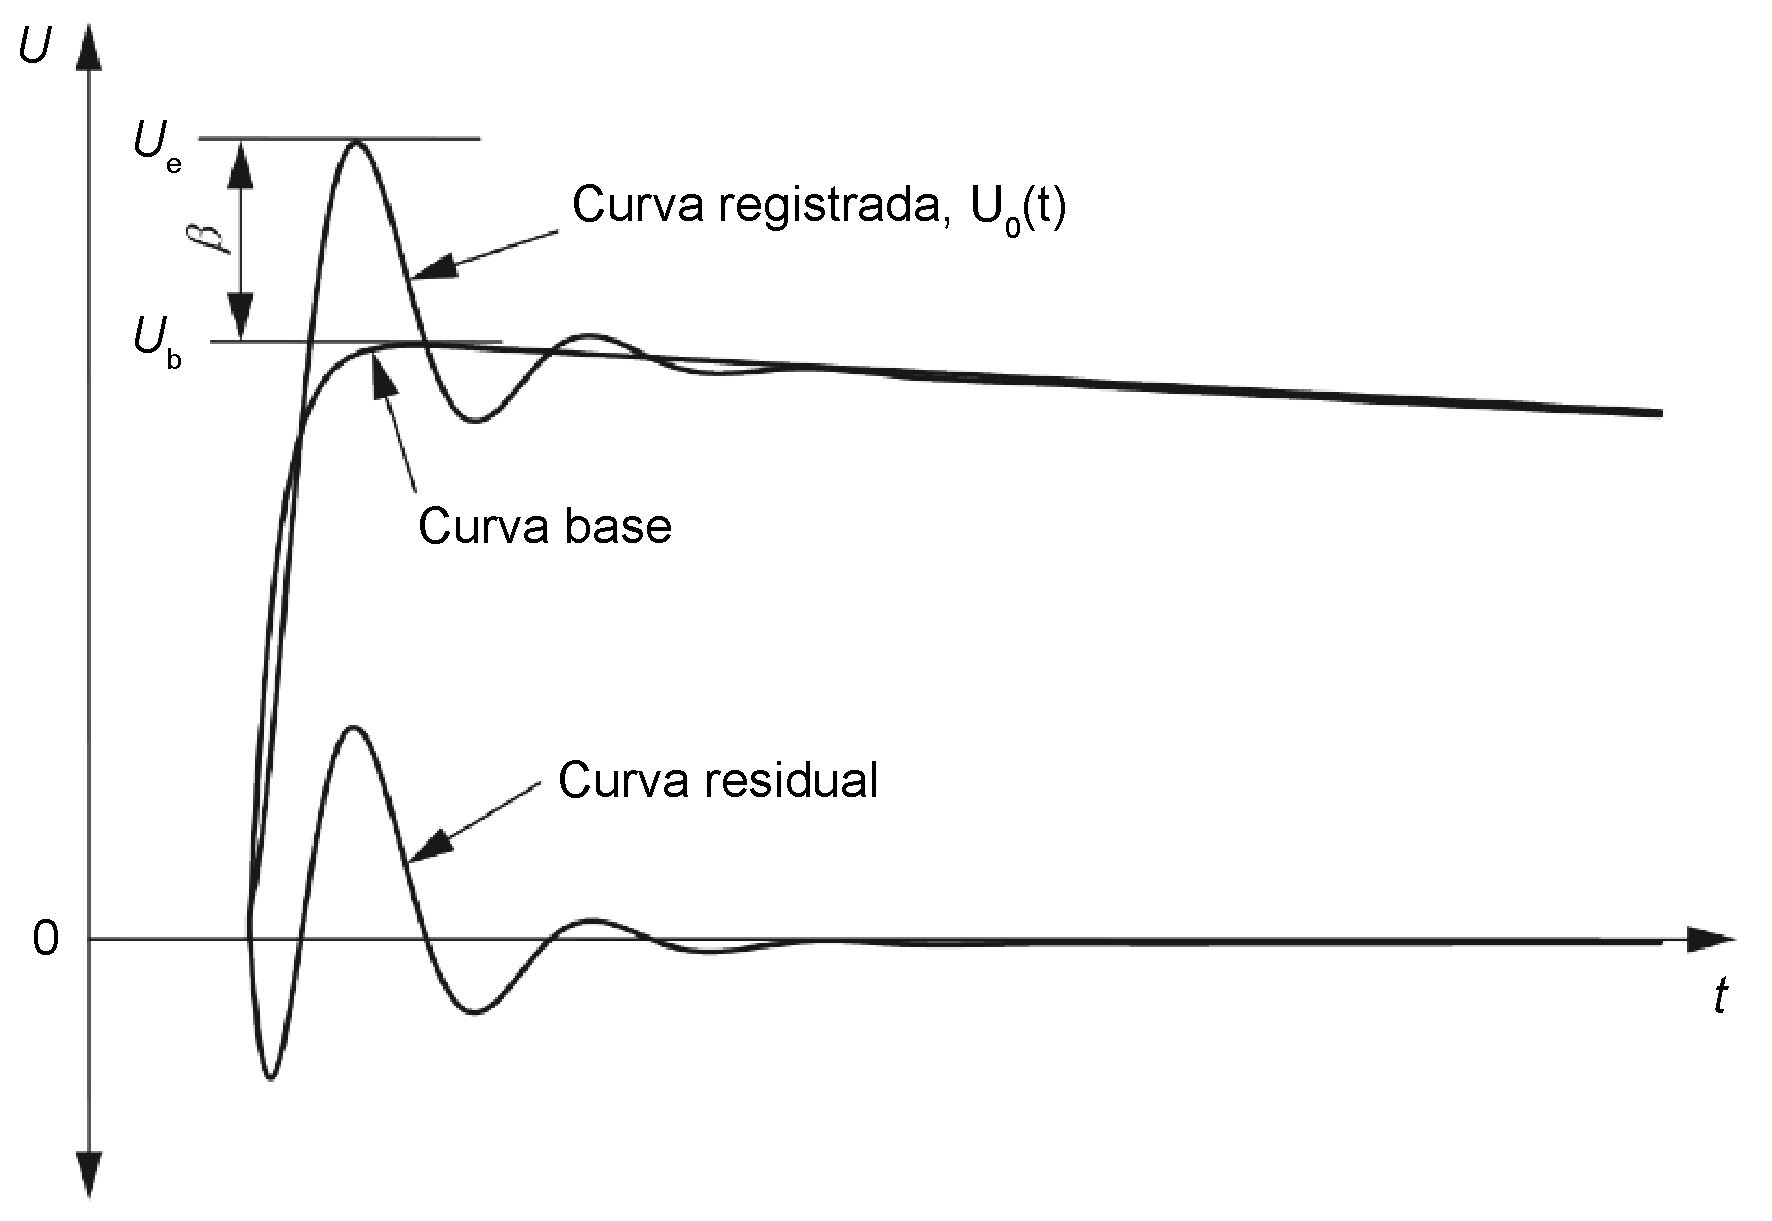
\includegraphics[width=1\textwidth]{img/iec_60060_1_curvas_registro_base_sobreimpulso_residual.png}
    \caption{Curva registrada con sobreimpulso, curva base y curva residual.}
    \label{fig:curvas_registro_base_sobreimpulso_residual}
\end{figure}

\textbf{Nivel de base:} Es el nivel de un registro de un sistema de medición de impulsos cuando hay una entrada cero al instrumento de registro.

\textbf{Curva base $U_\text{m}(t)$:} Es una estimación de una tensión de impulso tipo rayo completa sin una oscilación superpuesta.

\textbf{Curva residual $R(t)$:} Es la diferencia entre la curva registrada y la curva base.

\textbf{Valor extremo $U_\text{e}$:} Es el valor máximo de la curva registrada medido desde el nivel de base en el mismo sentido que el impulso aplicado.

\textbf{Máximo de la curva base $U_\text{b}$:} Es el valor máximo de la curva base.

\textbf{Función de tensión de ensayo:} Es una función de amplitud-frecuencia que se define para representar la respuesta del aislamiento a impulsos con sobreelevación (\emph{overshoot}), dada por la ecuación \ref{eq:func_tension_ensayo}, donde $f$ es la frecuencia en \unit{\mega\hertz}.

\begin{equation}
        k(f) = \frac{1}{1+2,2 \cdot f^2}
        \label{eq:func_tension_ensayo}
\end{equation}
Nota: Aplicar esta función como un filtro paso bajo a la curva de tensión residual, permite el cálculo del valor de la tensión de ensayo de la tensión de impulso tipo rayo completa equivalente.
\begin{figure}[H]
    \centering
    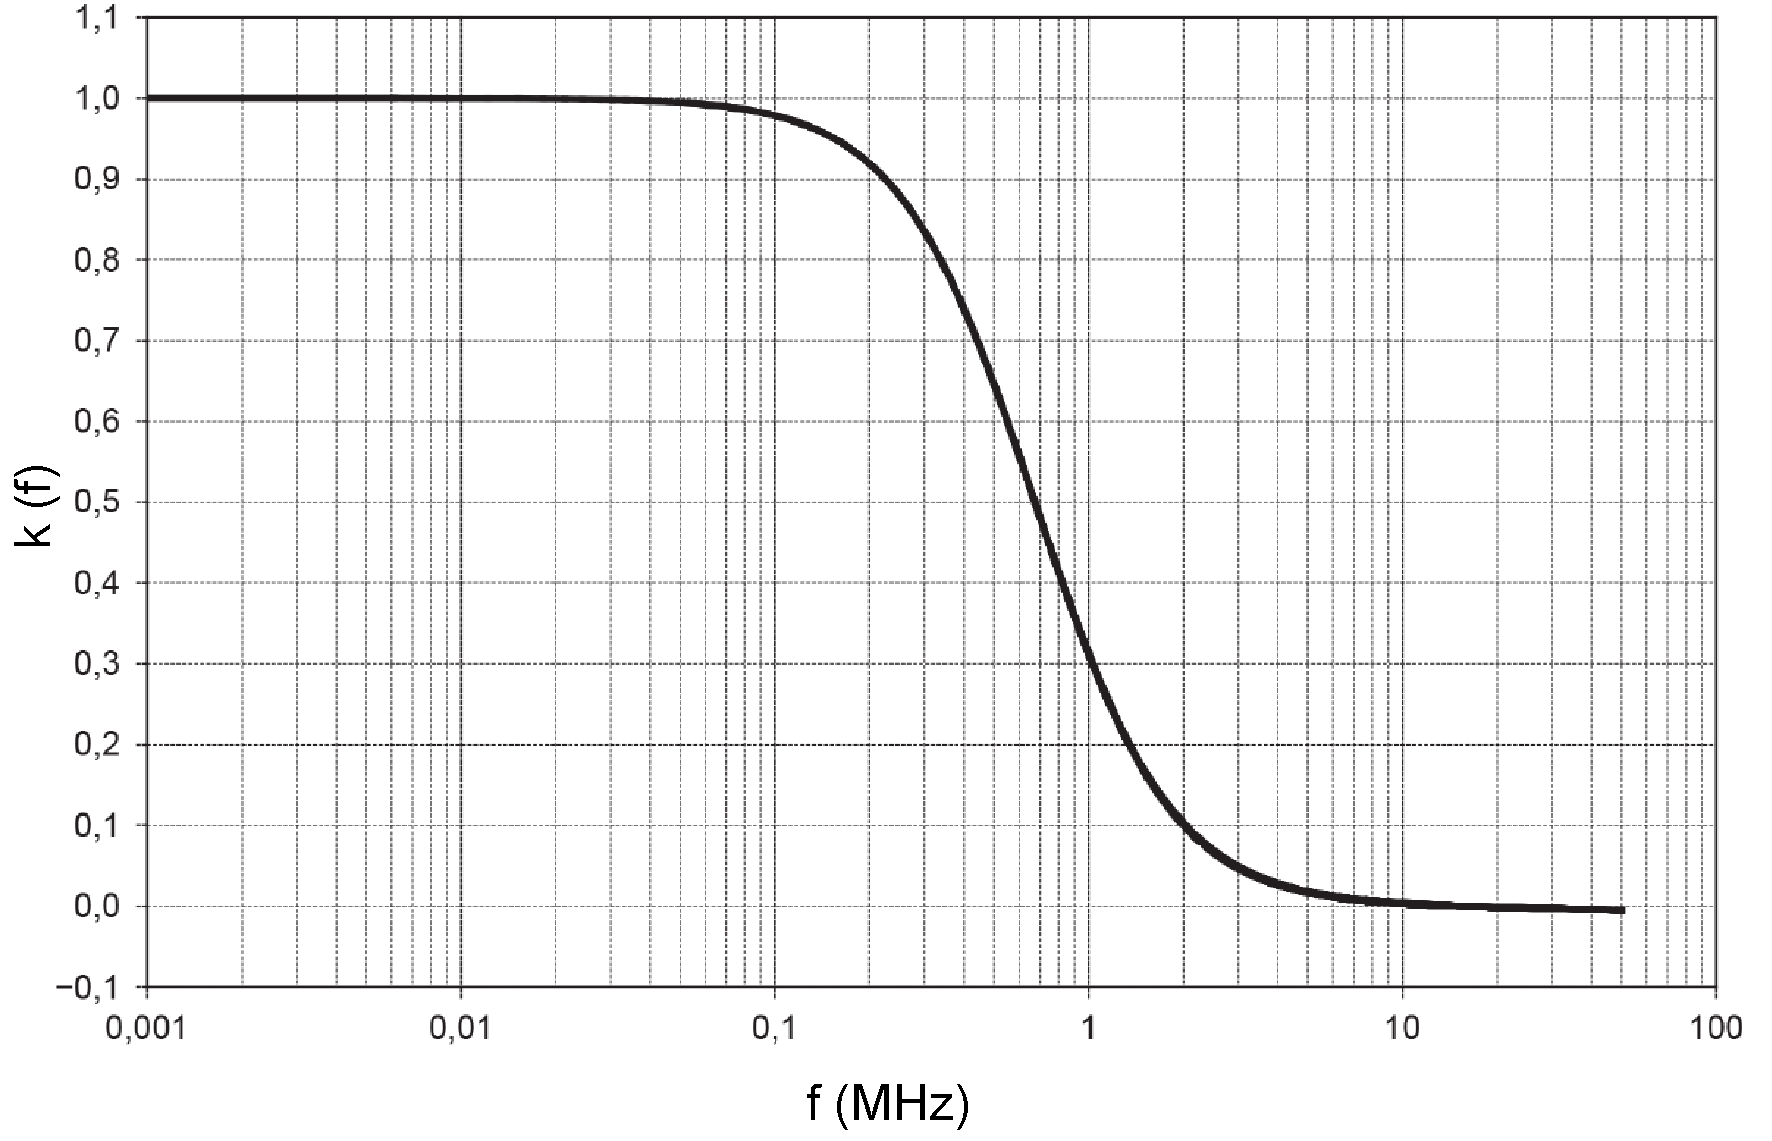
\includegraphics[width=1\textwidth]{img/iec_60060_1_funcion_tension_ensayo.png}
    \caption{Función tensión de ensayo.}
    \label{fig:funcion_tension_ensayo}
\end{figure}

\textbf{Curva residual filtrada ($R_f(t)$):} Es la curva residual filtrada por la función de tensión de ensayo de la ecuación \ref{eq:func_tension_ensayo}.
\begin{figure}[H]
    \centering
    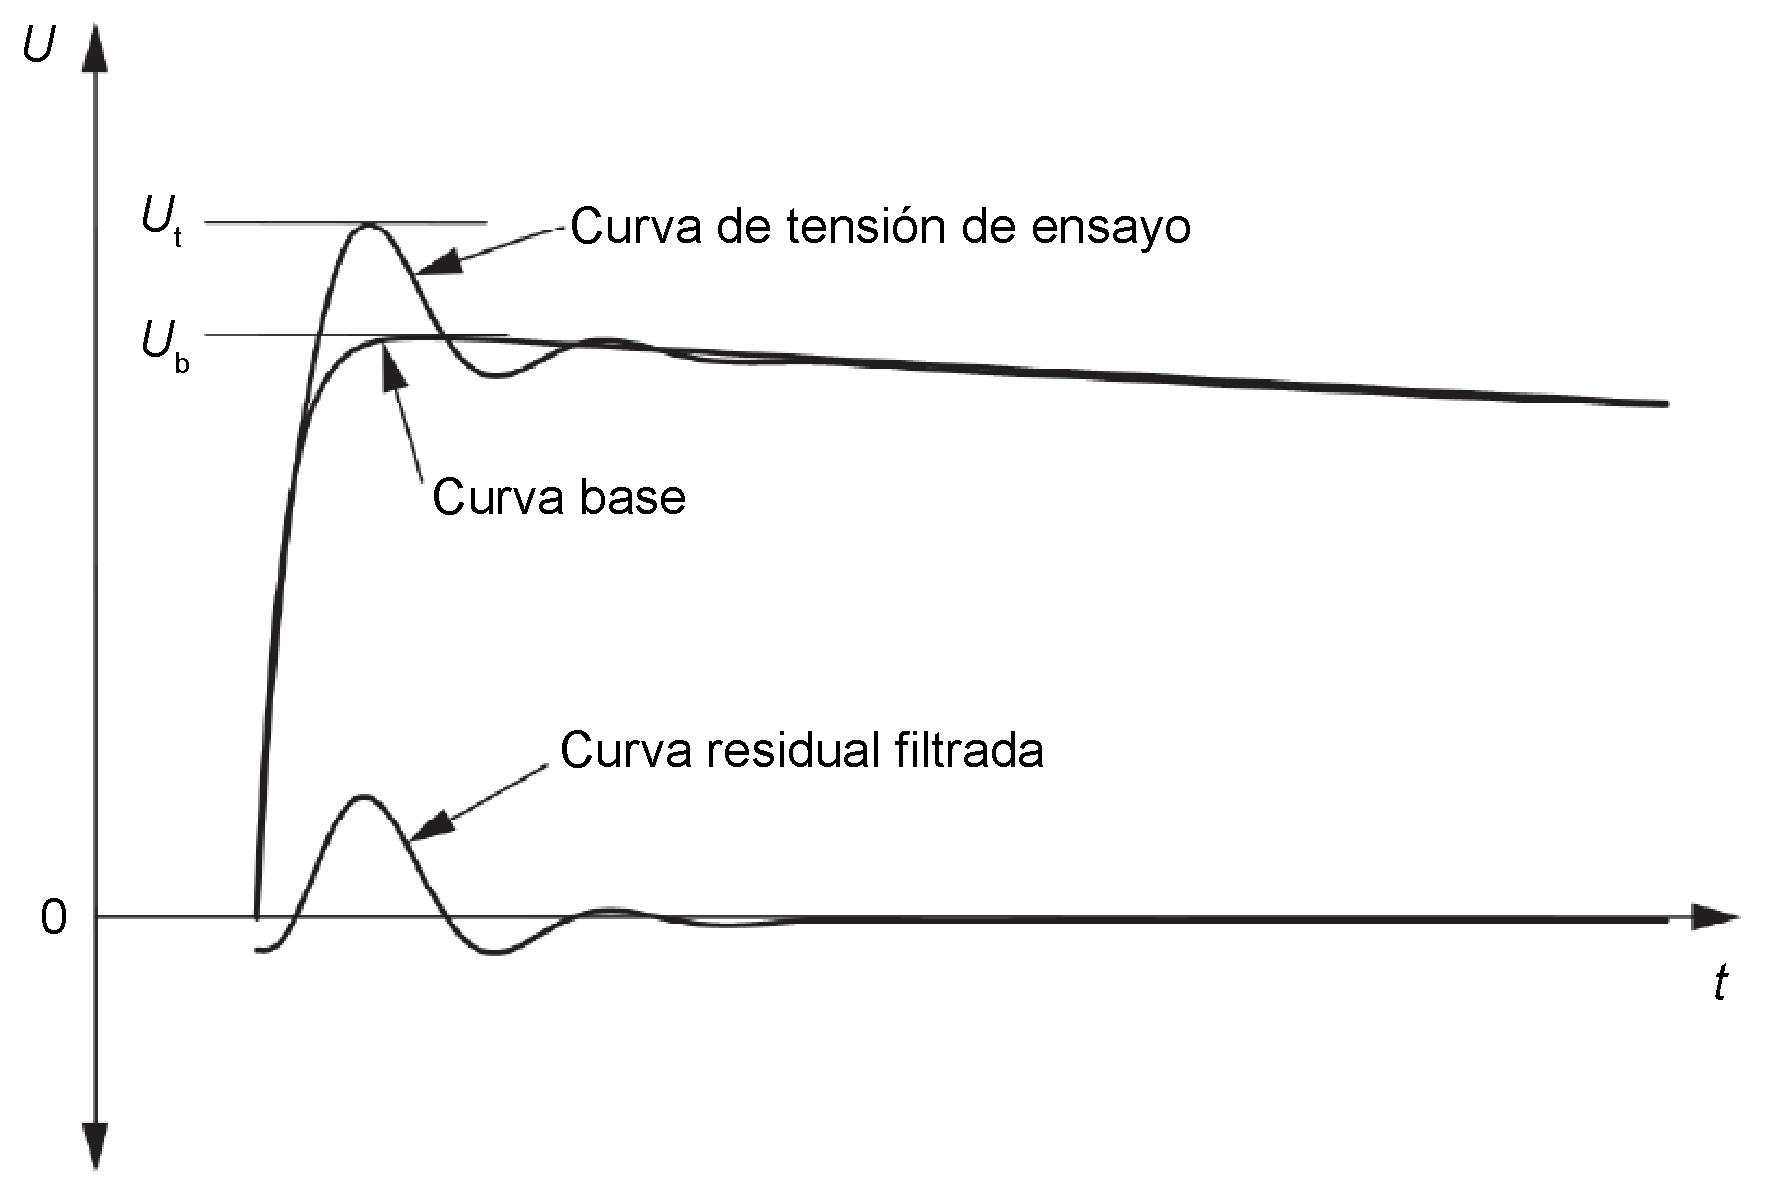
\includegraphics[width=1\textwidth]{img/iec_60060_1_curva_ensayo_base_filtrada.png}
    \caption{Curva tensión de ensayo (suma de curva base y curva residual filtrada).}
    \label{fig:curva_ensayo_base_filtrada}
\end{figure}

\textbf{Curva de tensión de ensayo:} Es la suma de la curva base con la curva residual filtrada. Es una representación matemática del proceso de filtrado y no es una entidad física o un impulso equivalente.
\begin{figure}[H]
    \centering
    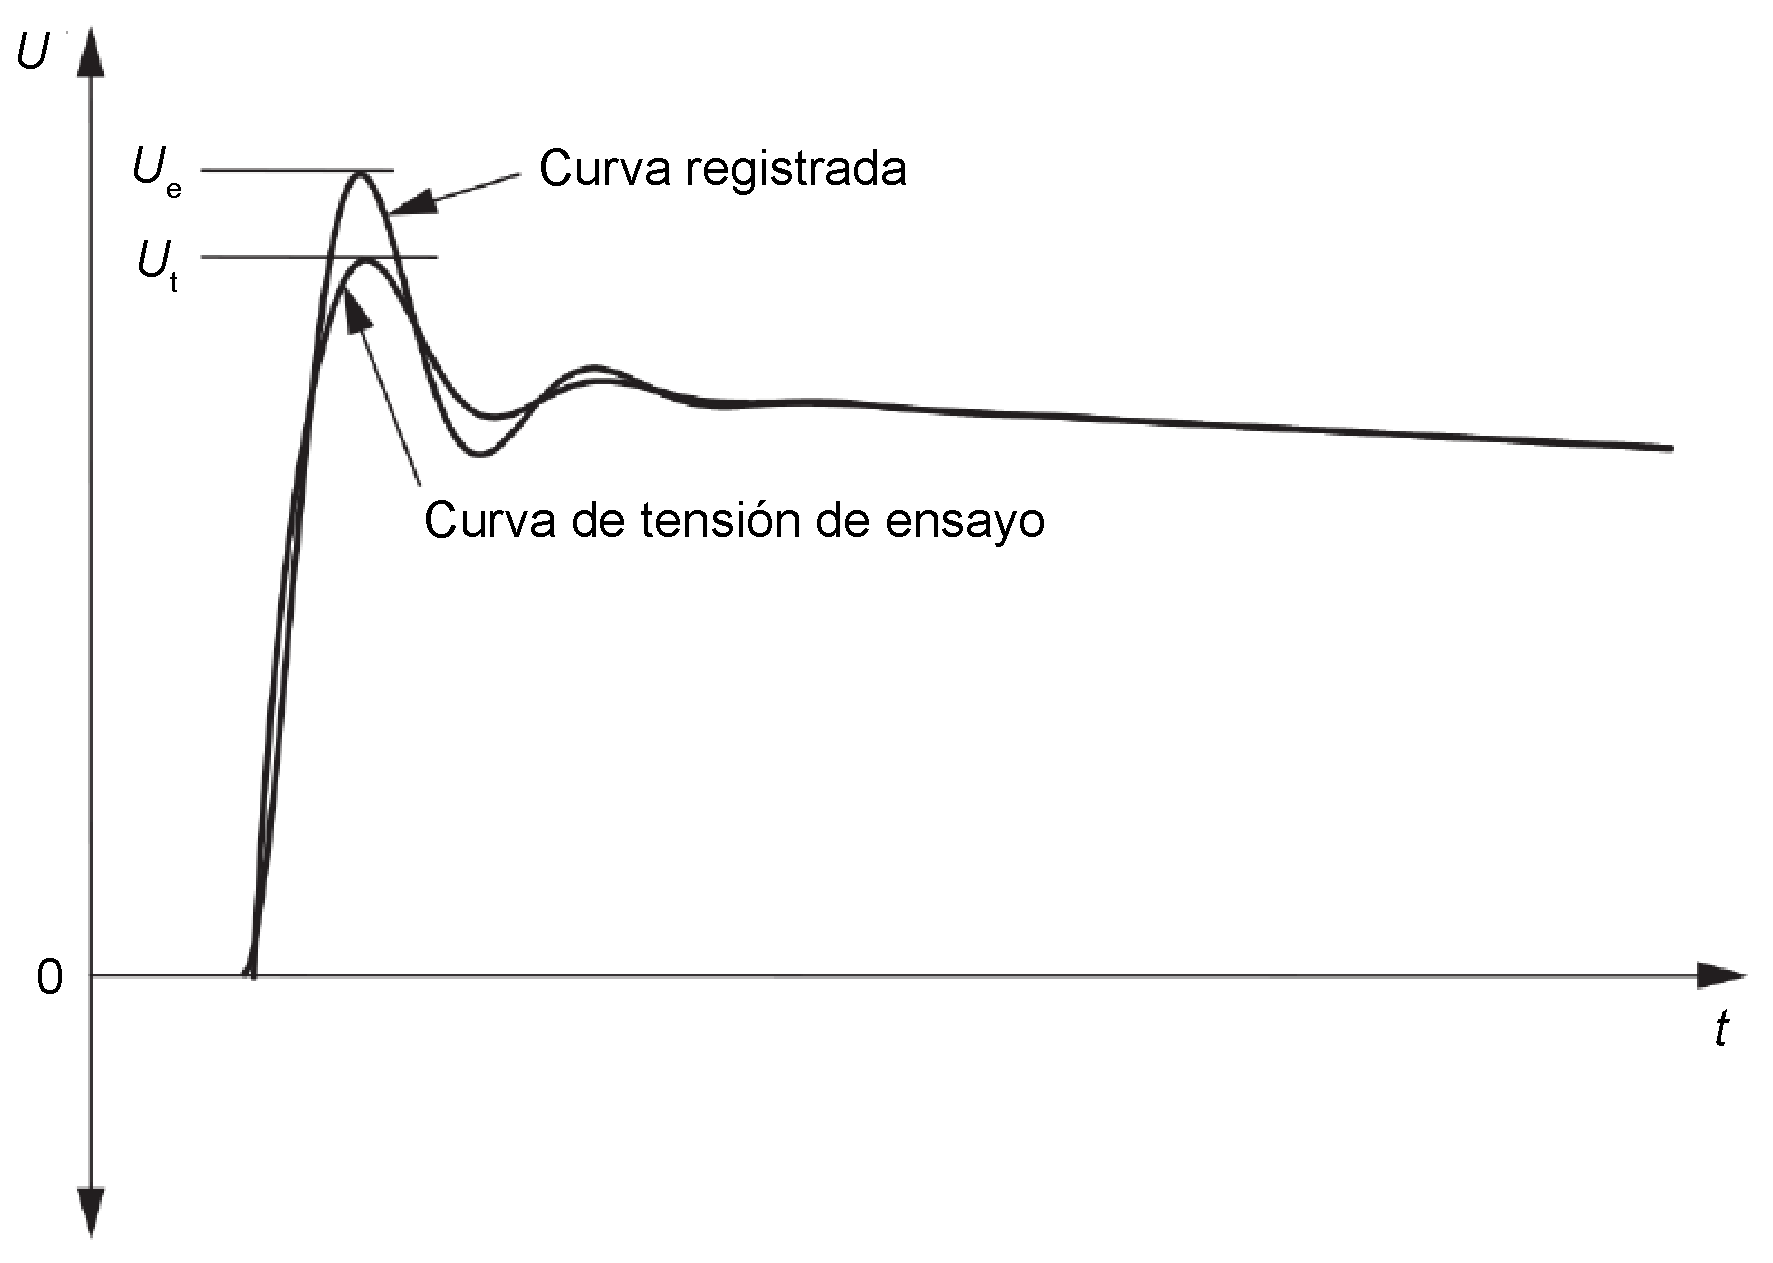
\includegraphics[width=1\textwidth]{img/iec_60060_1_curvas_ensayo_registrada.png}
    \caption{Curva tensión de ensayo y curva registrada.}
    \label{fig:curvas_ensayo_registrada}
\end{figure}

\textbf{Valor de la tensión de ensayo $U_\text{t}$:} Es el valor máximo de la curva de tensión de ensayo, medido desde el nivel de base en el mismo sentido que el impulso aplicado.

\textbf{Magnitud de la sobreelevación $\beta$:} Es la diferencia entre el valor extremo de la curva registrada ($U_\text{e}$) y el valor máximo de la curva base ($U_\text{b}$).

\textbf{Magnitud relativa de la sobreelevación $\beta'$:} Es la relación porcentual entre la magnitud de la sobreelevación y el valor extremo.

\textbf{Tiempo de frente $T_1$:} Es un parámetro virtual definido como $1/0,6$ veces el intervalo $T_{AB}$ entre los instantes en que el impulso es \qty{30}{\percent} y \qty{90}{\percent} del valor de cresta en la curva de tensión de ensayo.

\begin{equation}
    T_1 = \frac{T_{AB}}{0,6} = \frac{t_{90} - t_{30}}{0,6}
    \label{eq:tiempo_frente}
\end{equation}

\begin{figure}[H]
    \centering
    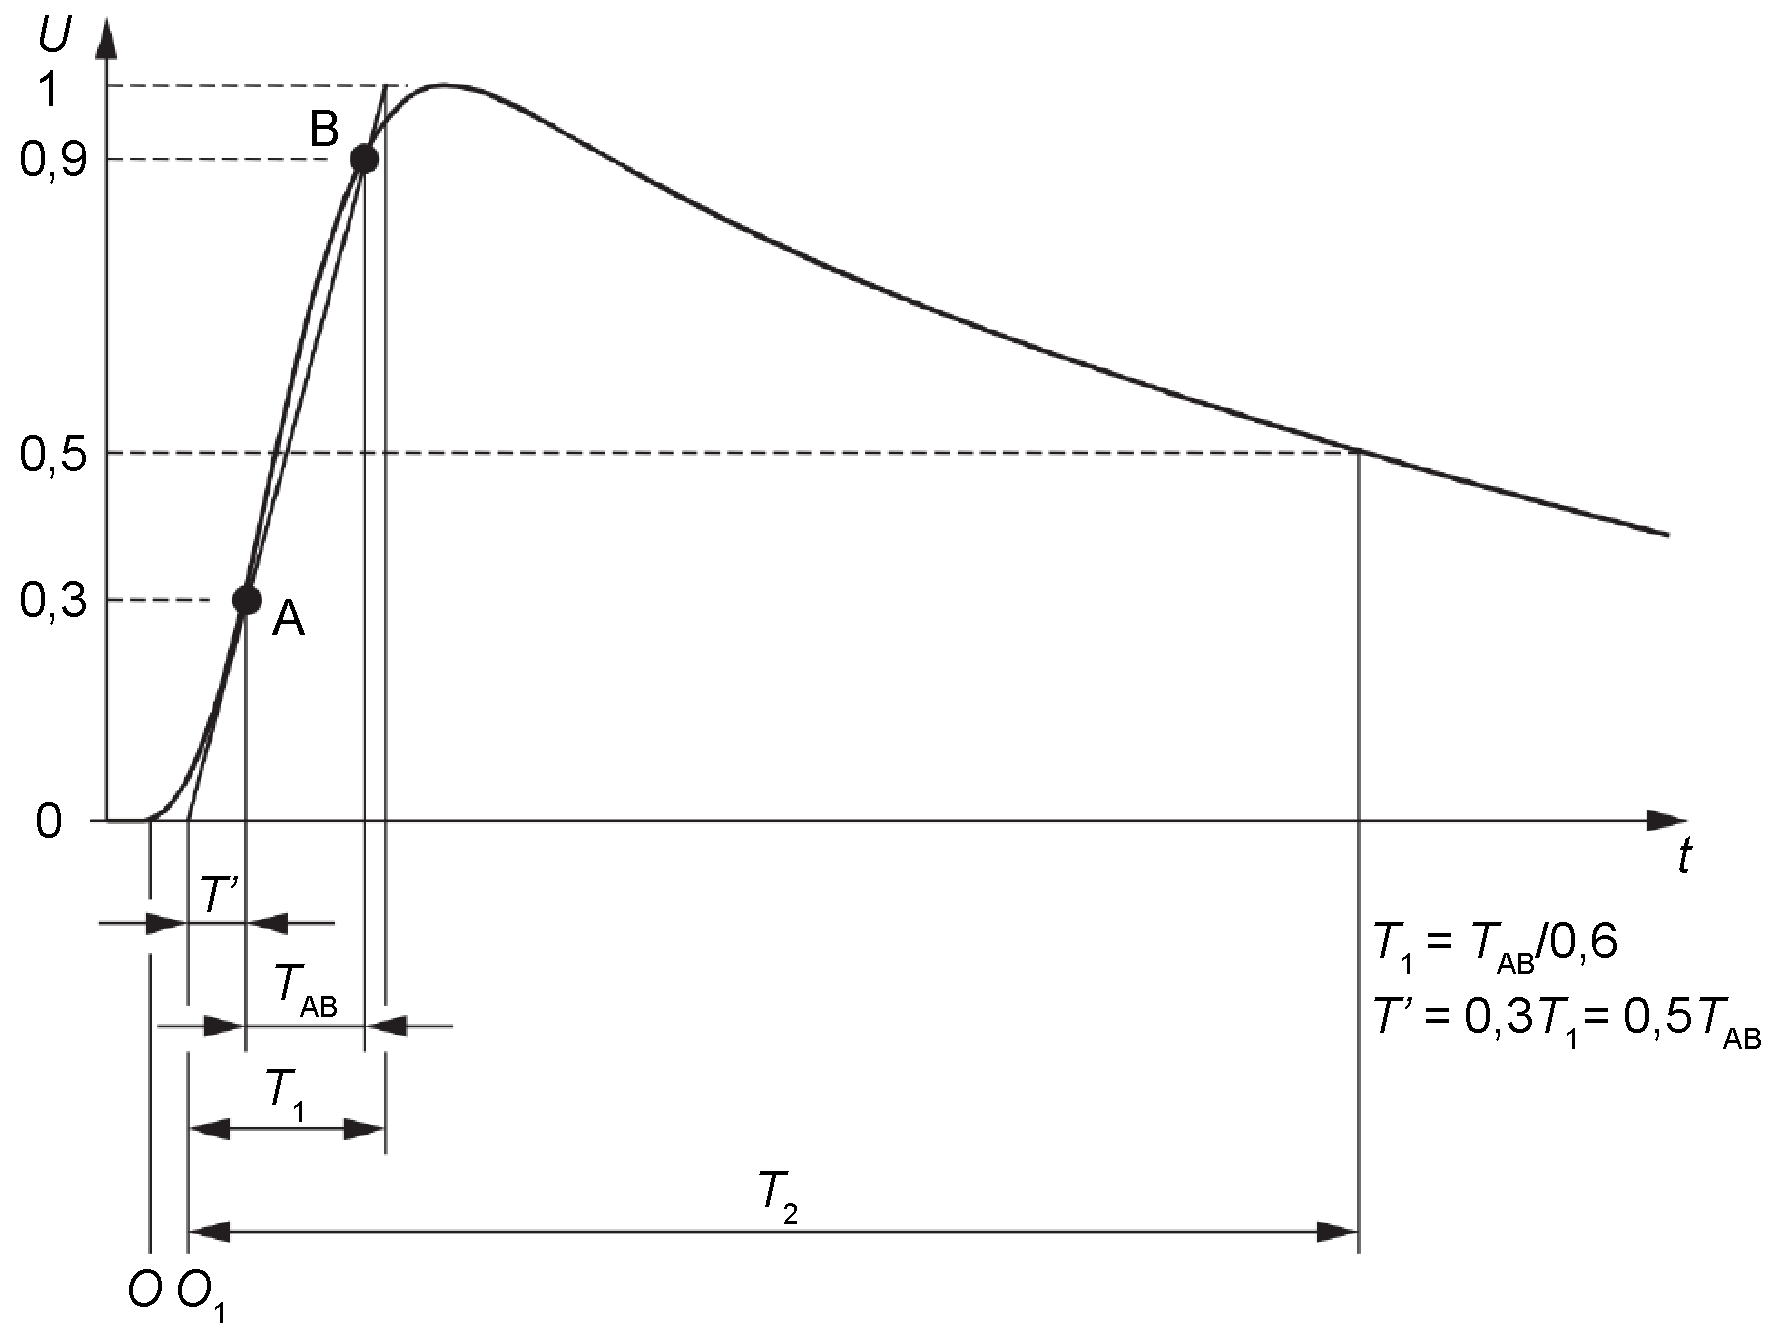
\includegraphics[width=1\textwidth]{img/iec_60060_1_parametros_temporales_impulso_pleno.png}
    \caption{Parámetros de tiempo del impulso de tensión tipo rayo pleno.}
    \label{fig:parametros_temporales_impulso_pleno}
\end{figure}

\textbf{Origen virtual $O_1$:} Es un instante que precede al punto A de la curva de tensión de ensayo en un tiempo $0,3 * T_1$.
\begin{align}
    T' &= 0.5 \cdot T_{AB} \\
    T' &= 0.5 \cdot 0.6 \cdot T_1 \\
    T' &= 0.3 \cdot T_1
    \label{eq:t_prima}
\end{align}
Luego:
\begin{equation}
    O_1 = t_{30} - 0.3 \cdot T_1 = t_{30} - 0.5 \cdot T_{AB}
    \label{eq:origen_virtual}
\end{equation}

\textbf{Tiempo hasta el semi-valor $T_2$:} Es un parámetro virtual definido como el intervalo de tiempo entre el origen virtual ($O_1$), y el instante en que la curva de tensión de ensayo disminuye a la mitad del valor de cresta de la tensión de ensayo ($U_\text{t}$).

\textbf{Tensión de impulso tipo rayo cortada:} Es un impulso tipo rayo que es interrumpido en el frente, cresta o cola por una descarga disruptiva, causando una caída súbita de la tensión.

\textbf{Instante de corte:} Es el instante en el que la extrapolación de la línea entre los puntos del \qty{70}{\percent} y \qty{10}{\percent} (C y D) en el colapso de la tensión cruza el nivel inmediatamente anterior al colapso.
\begin{figure}[H]
    \centering
    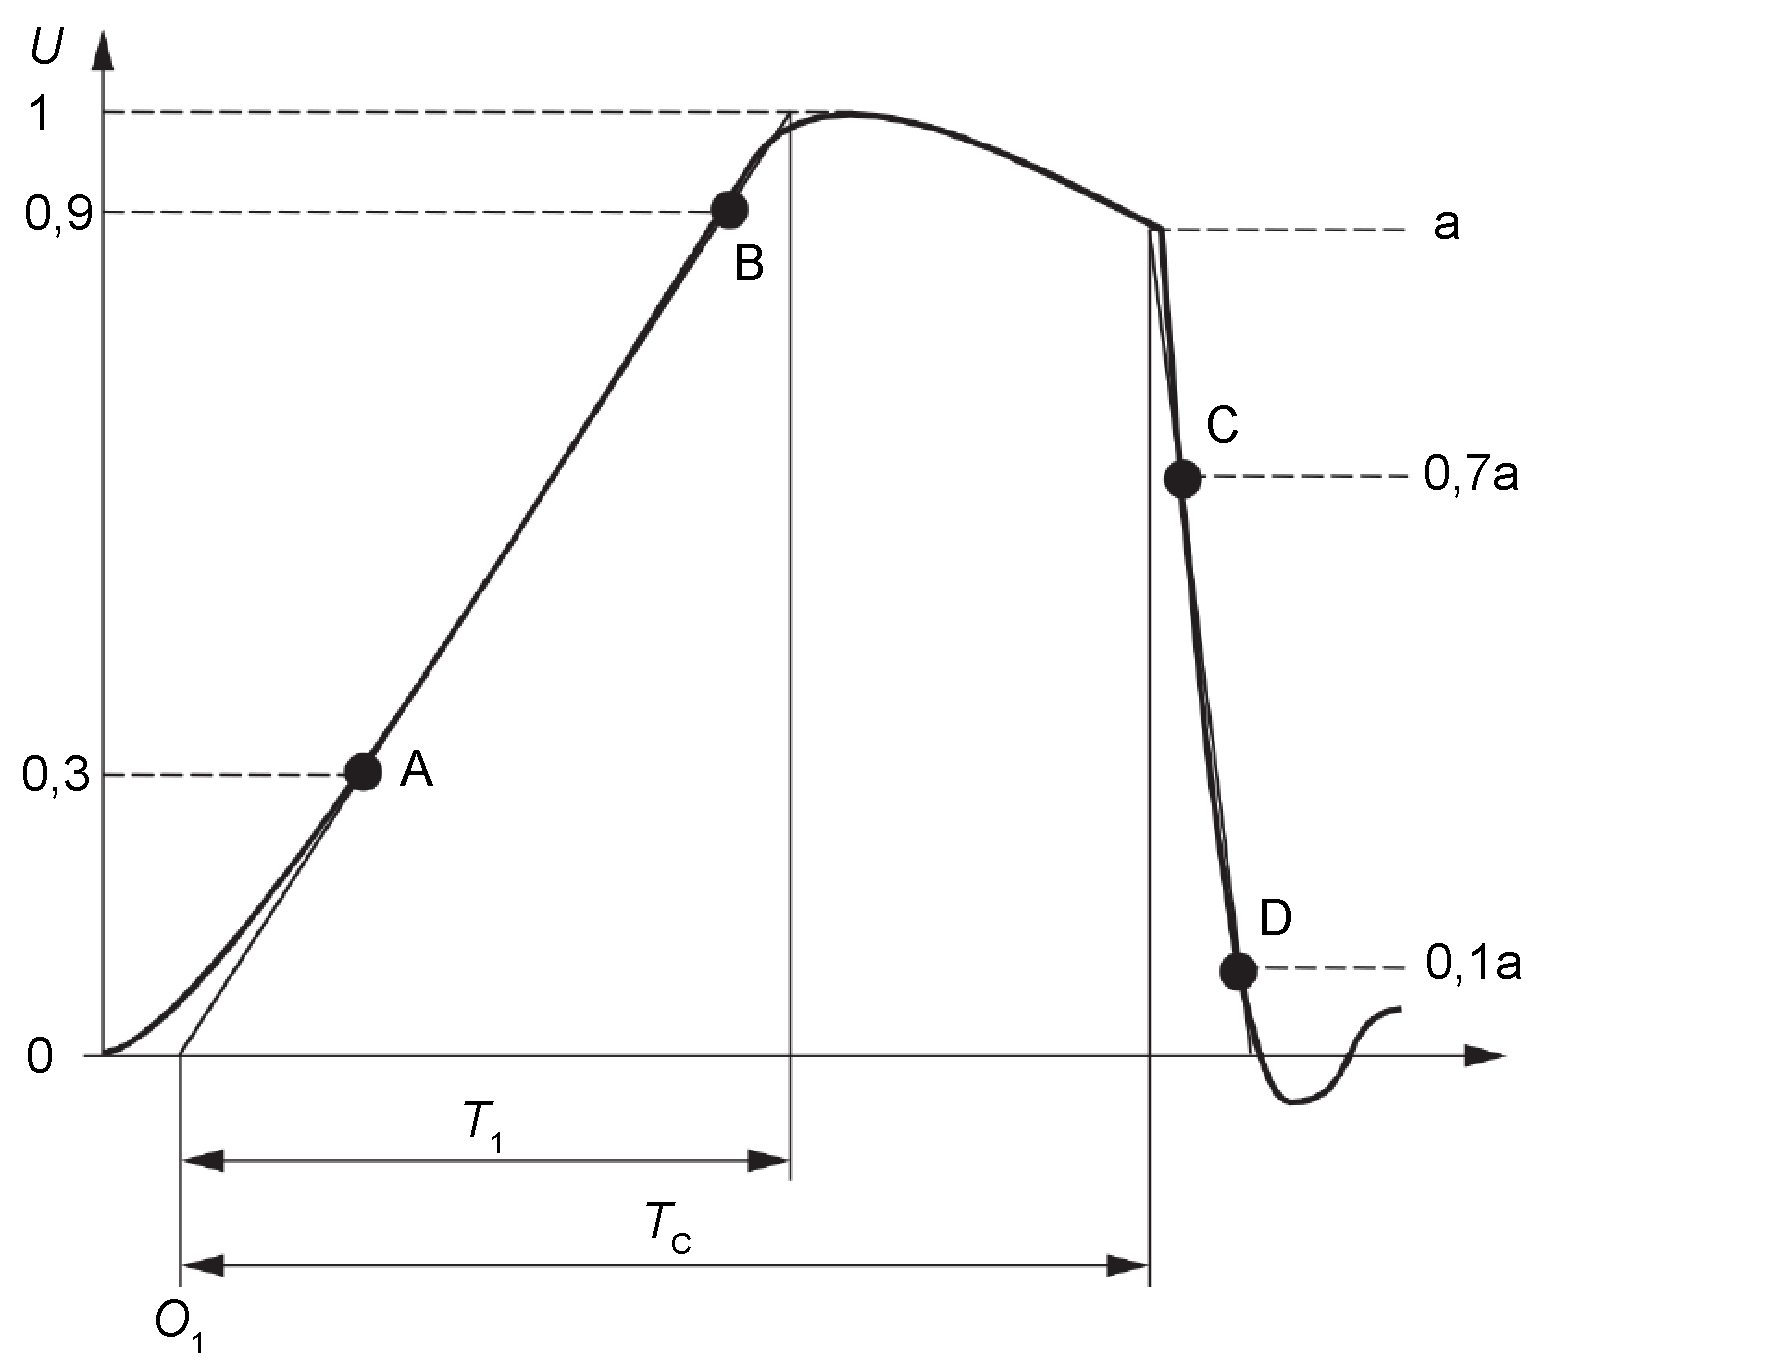
\includegraphics[width=1\textwidth]{img/iec_60060_1_impulso_tension_cortado_cola.png}
    \caption{Impulso de tensión tipo rayo cortado en la cola.}
    \label{fig:impulso_tension_cortado_cola}
\end{figure}

\textbf{Tiempo de corte $T_\text{C}$:} Es el intervalo de tiempo entre el origen virtual ($O_1$) del impulso y el instante relevante.

\subsection{Onda de impulso plena}

Según la norma IEC 60060-1 \cite{iec60060_1}, la tensión de impulso tipo rayo estándar u \enquote{Onda plena} es una tensión de impulso tipo rayo completa y suave, que tiene un tiempo de frente ($T_1$) de \qty{1,2}{\micro\second}, y un tiempo hasta el semi-valor ($T_2$) de \qty{50}{\micro\second}, y se denomina impulso \qty[parse-numbers=false]{1,2/50}{\micro\second}.

Además, la norma establece las tolerancias que acepta en los parámetros característicos, indicados en la tabla \ref{tab:tolerancias_impulso}:

\begin{table}[H]
    \centering
    \caption{Tolerancias de la onda de impulso según IEC 60060-1.}
    \label{tab:tolerancias_impulso}
    \begin{tabular}{@{}ll@{}}
        \toprule
        \textbf{Parámetro}                 & \textbf{Tolerancia}                                                                                     \\ \midrule
        Tensión de ensayo ($U_\text{t}$)   & $\pm \qty{3}{\percent}$                                                                                 \\ \midrule
        Tiempo de frente ($T_1$)           & $\pm \qty{30}{\percent}$                                                                                \\
                                           & y para equipos con $U_\text{m} > \qty{800}{\kilo\volt}$: $\qty{-30}{\percent}$ a $+\qty{100}{\percent}$ \\ \midrule
        Tiempo hasta el semi-valor ($T_2$) & $\pm \qty{20}{\percent}$                                                                                \\ \midrule
        Sobreelevación (OS)                & $\le \qty{10}{\percent}$                                                                                \\ \bottomrule
    \end{tabular}
\end{table}

\subsection{Onda de impulso cortada}

Un impulso tipo rayo estándar cortado u \enquote{Onda cortada}, se denomina así cuando es interrumpido por un entrehierro externo con un tiempo de corte ($T_\text{C}$) entre \qty{2}{\micro\second} y \qty{5}{\micro\second}. Las características del colapso de tensión durante el corte se determinan por el instante del valor \qty{70}{\percent} y \qty{10}{\percent} de la tensión de impulso aplicada antes del colapso.
La duración del colapso de tensión debe ser mucho más rápida que el tiempo de frente ($T_1$) del impulso.

\section{Características del ensayo de impulso}

El ensayo de impulso es una prueba de alta tensión y corta duración, utilizada para verificar la rigidez dieléctrica y el aislamiento de equipos eléctricos, tales como, transformadores, seccionadores y celdas de media tensión, entre otros.

El impulso tipo rayo se produce mediante un generador de impulsos Marx, el cual consiste en un conjunto de capacitores que se cargan en paralelo desde una fuente de tensión continua de baja tensión, que luego se descargan en serie a través del objeto bajo ensayo.

El ensayo de impulso, se realiza aplicando una cierta cantidad de impulsos al objeto bajo ensayo (que dependen de la norma aplicable a dicho elemento), y registrando la respuesta del mismo, mediante un sistema de adquisición de datos, compuesto por un divisor de tensión (resistivo o capacitivo), un atenuador coaxial y un oscilocopio digital.

El análisis de los parámetros del impulso registrado permite evaluar la capacidad del equipo para soportar sobretensiones transitorias referidas a descargas atmosféricas, y determinar su rigidez dieléctrica.

Respecto al análisis de la onda, la norma IEC 60060-1 en su Anexo B, describe un método para el cálculo de los parámetros de las ondas de impulso tipo rayo estándar (plenas y cortadas) con o sin sobreelevación u oscilaciones superpuestas. Este método se basa en la estimación de una curva base, que representa la forma idealizada de un impulso tipo rayo sin oscilaciones, y el cálculo de una curva residual, que representa las oscilaciones superpuestas. Posteriormente, se aplica un filtro a la curva residual, definido por la función de tensión de ensayo (ecuación \ref{eq:func_tension_ensayo}) para luego, obtener la curva de tensión de ensayo, de la cual se calculan los parámetros del impulso. Mientras que, en el Anexo D de la misma norma, contiene una guía de implementación de software para la implementar el ajuste de la curva base, y el filtro digital con la función de tensión de ensayo (ecuación \ref{eq:func_tension_ensayo}).